\chapter{Experiment 2}

\textbf{Author: } 

The second experiment is performed for the reason of testing the neural network with images of real objects. This experiment is mandatory for testing the capabilities of the neural network when it comes to real images.

\section{Preparation}
The first step of the authors was choosing a suitable object. In an effort to be time efficient once again the monkey head was chosen. This had the advantage that 3D-printing the object was easy, as all the authors had to do was exporting the existing model from Blender, and, even better, the trained weights of this object were already existing. Next the 3D model of the head was modified to include a cylindrical hole at the bottom, be able to easily mount the object. The last step was printing the object with a 3D printer. For this a Ultimaker Original and pink PLA (Polylactic acid) filament was used.

\section{Setup and Environment}
The setup consisted of a Parrot Bebop 2 and the 3D printed monkey head put on a stick to simulate the height of the head in the images produced by Blender. The authors chose a mostly white background, consisting of a table and a painted wooden board leaned on the table.

The authors were not specific about the lighting, because this experiment was to be performed as realistic as possible. For example in drone competitions the lighting often can not be influenced.

The monkey head was placed on the table facing away from the white wooden board. The drone was positioned at a distance of approximately 14cm from the object. The drone's camera was looking directly towards the object. After taking the first image the drone was moved to a second position, again about 14cm away and looking at the object. This resulted in the drone rotating slightly to the left to keep the object centred.

\section{Sequence of Events}

\begin{figure*}[h!]
	\centering
	\begin{subfigure}[t]{\textwidth}
		\centering
		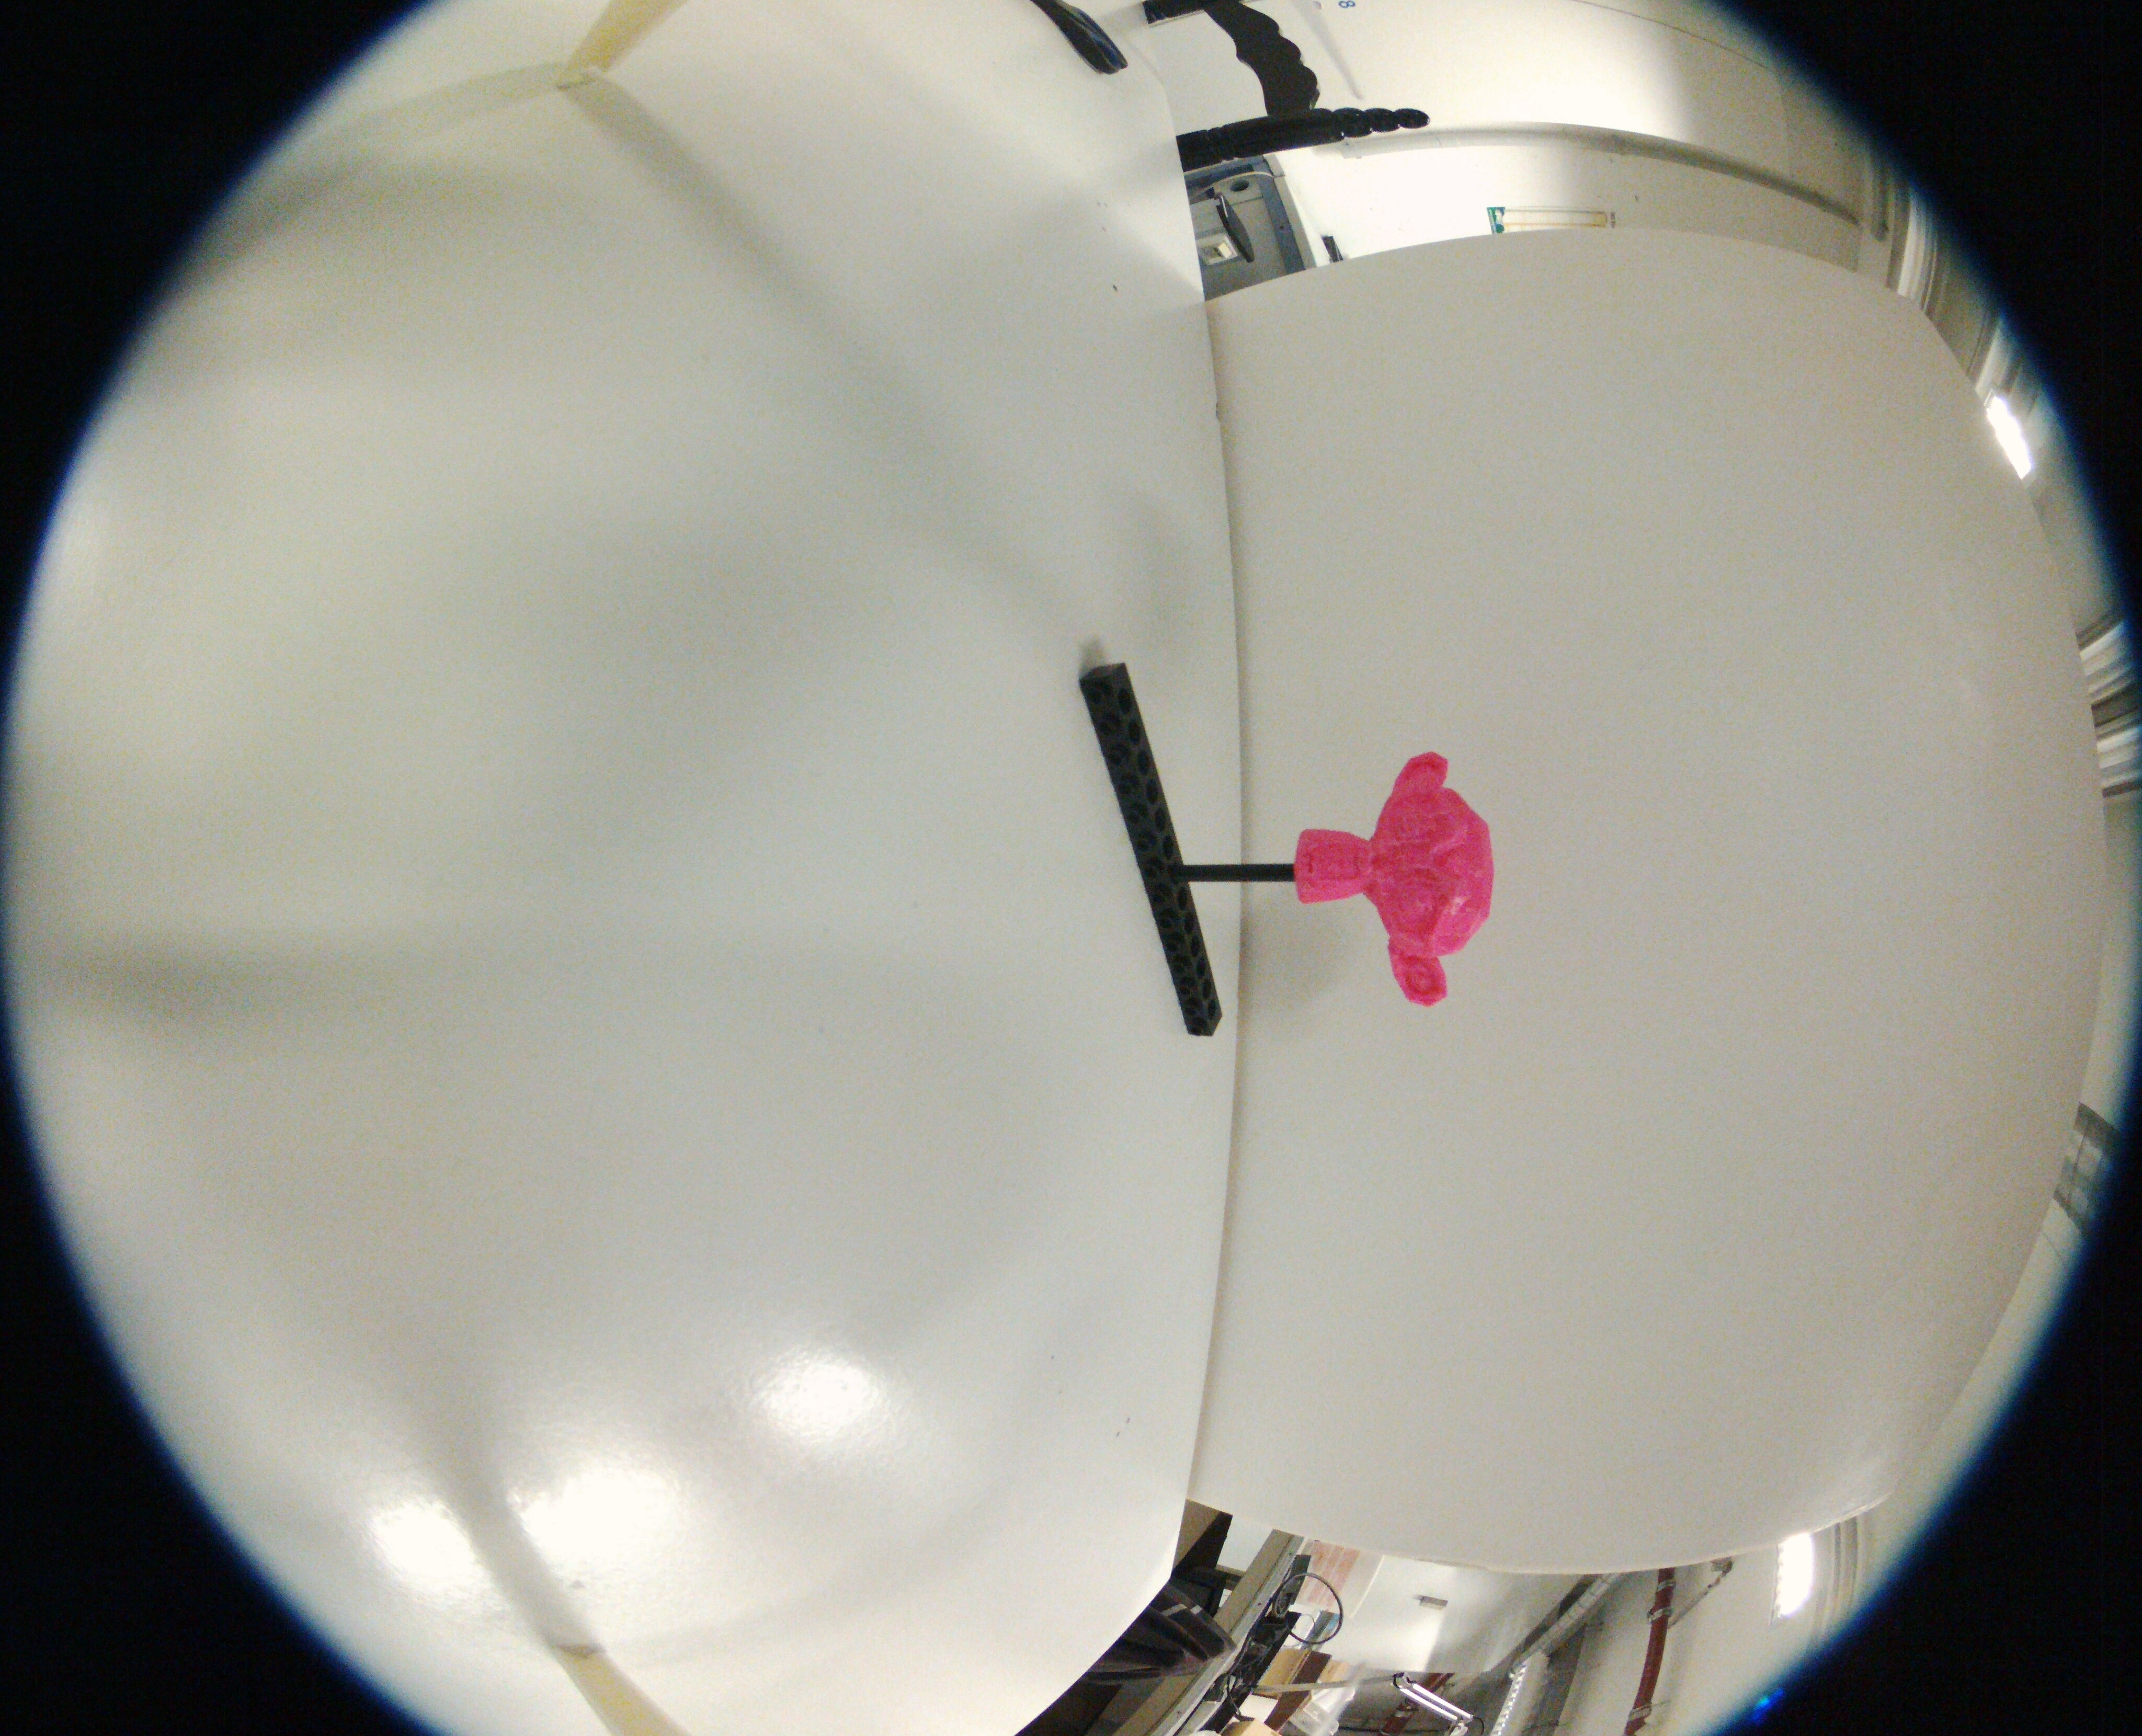
\includegraphics[width=0.48\textwidth]{img/experiment1_original_bebop_img_1.jpg}
		\hfill
		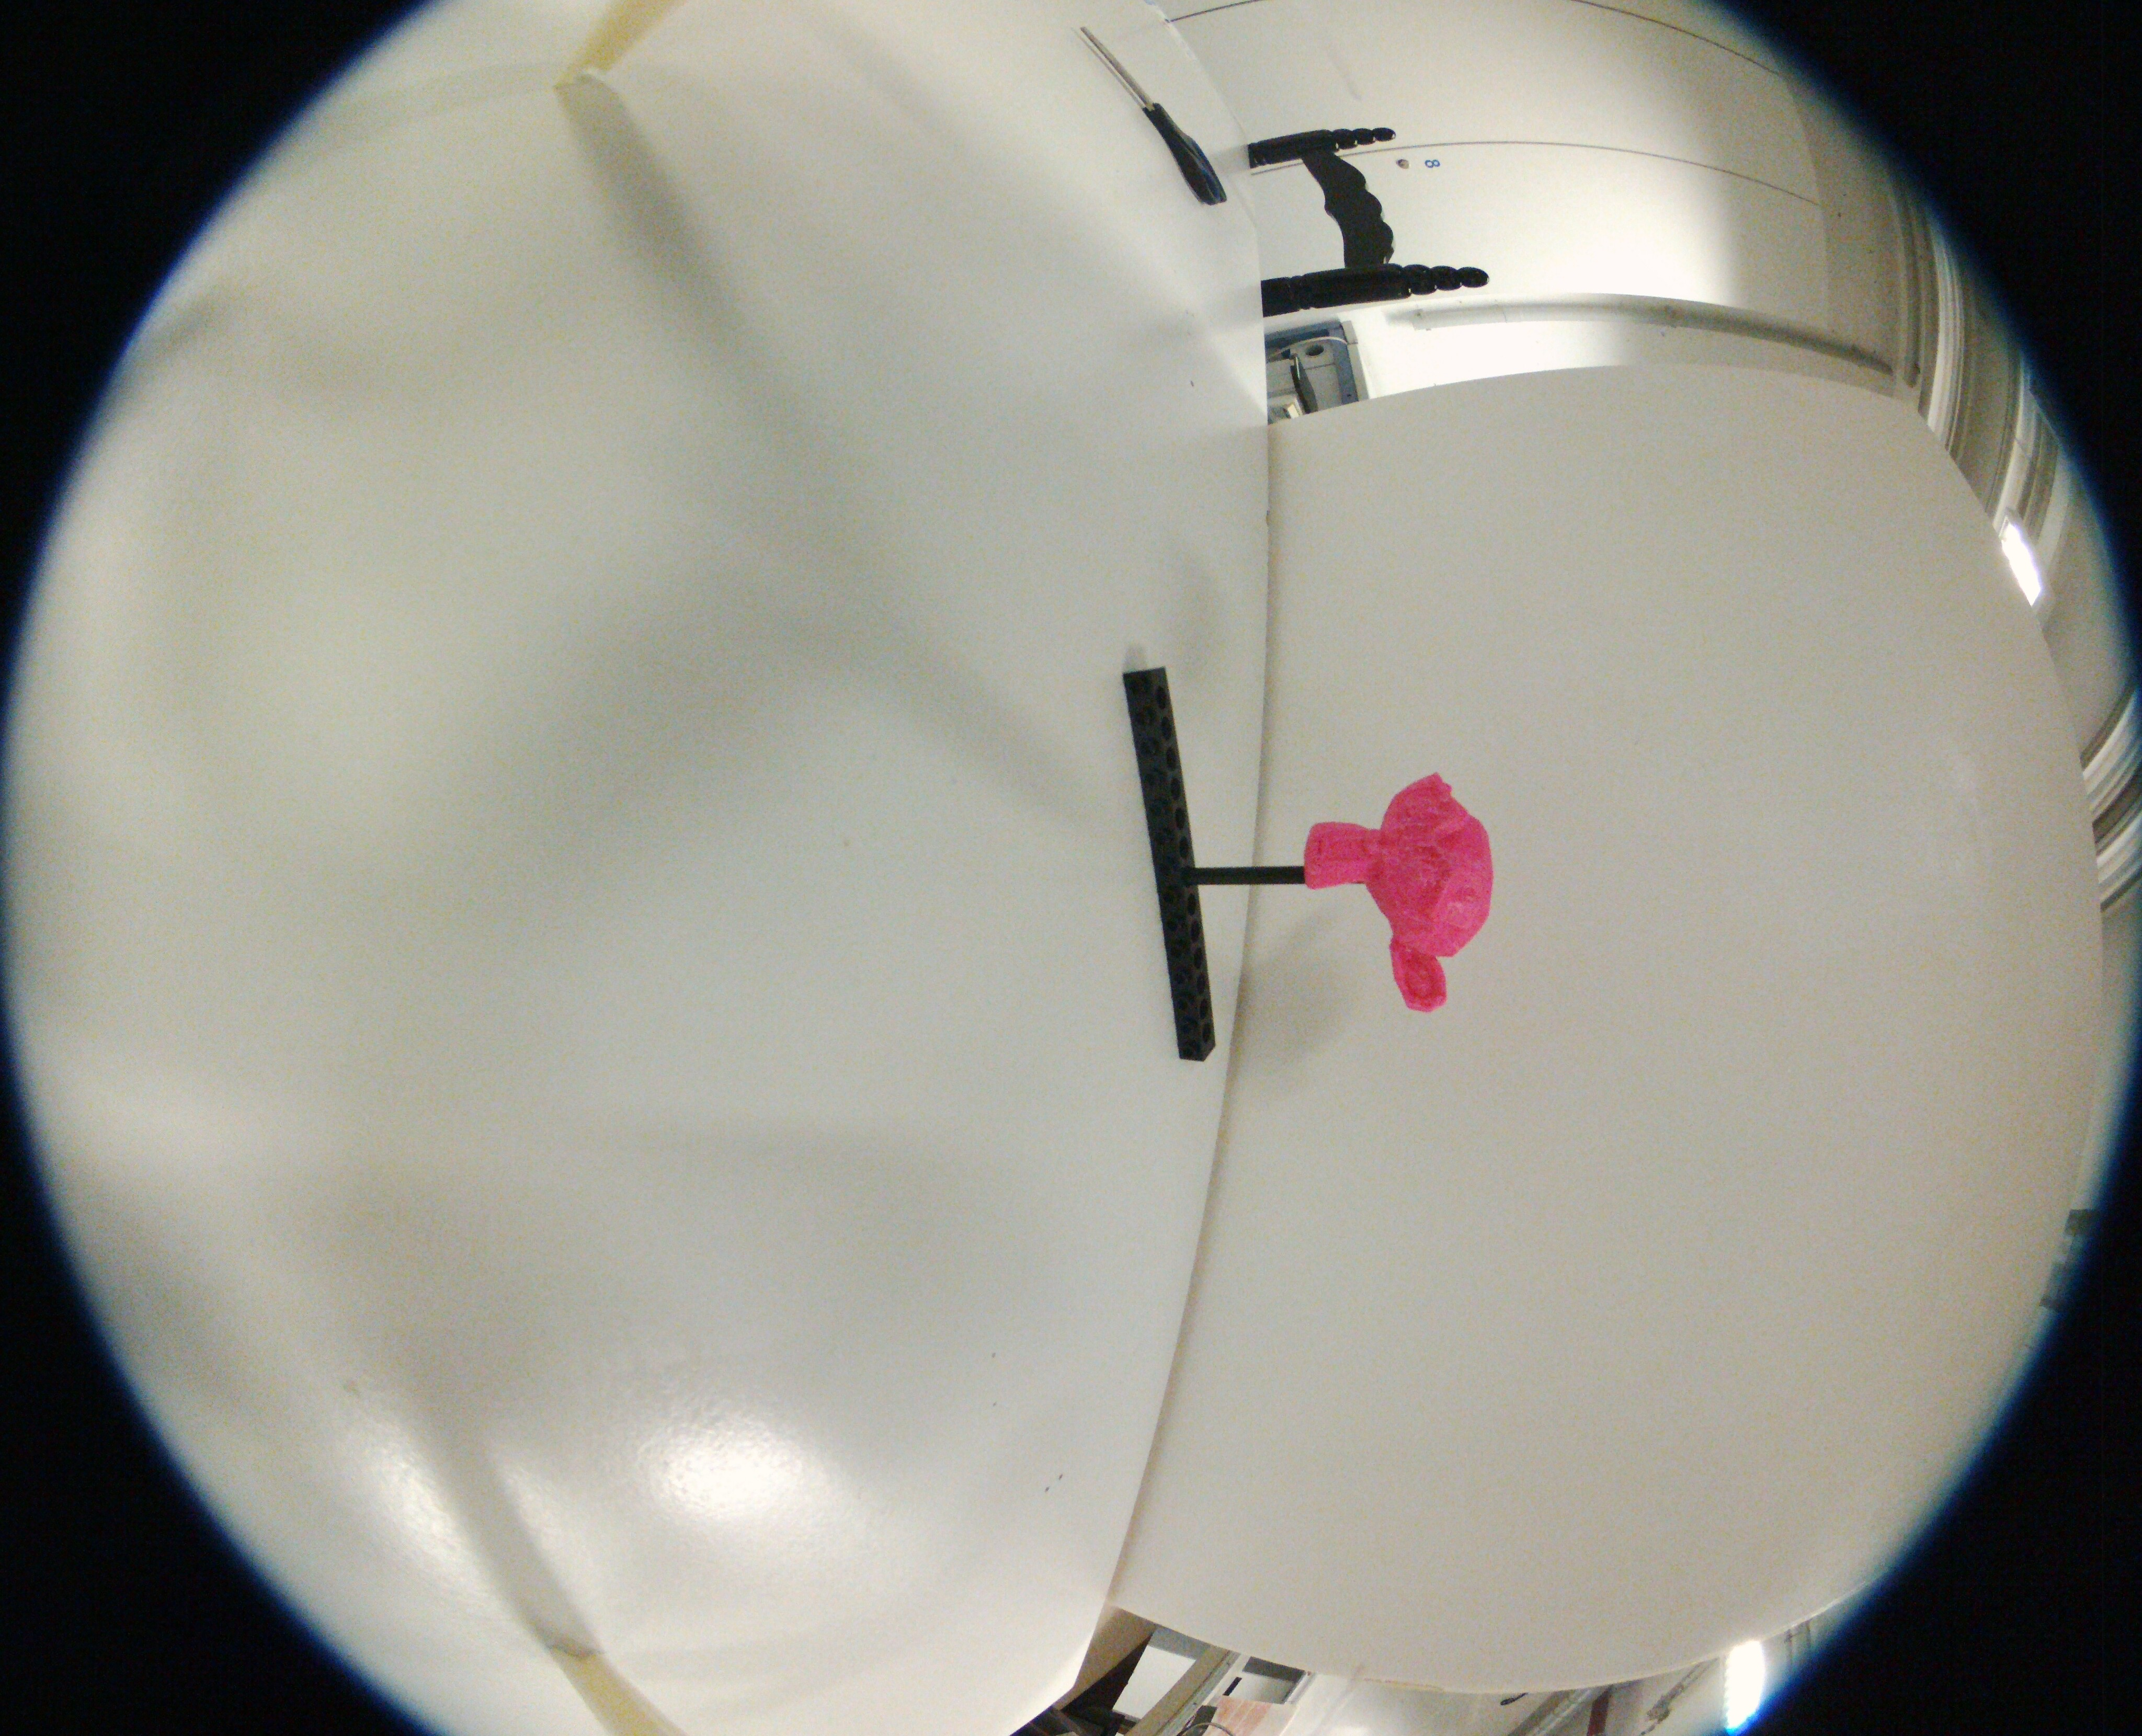
\includegraphics[width=0.48\textwidth]{img/experiment1_original_bebop_img_2.jpg}
		\caption{The original images of the 3D printed monkey head produced by the Parrot~Bebop~2.}
	\end{subfigure}
	~ 
	\begin{subfigure}[t]{\textwidth}
		\centering
		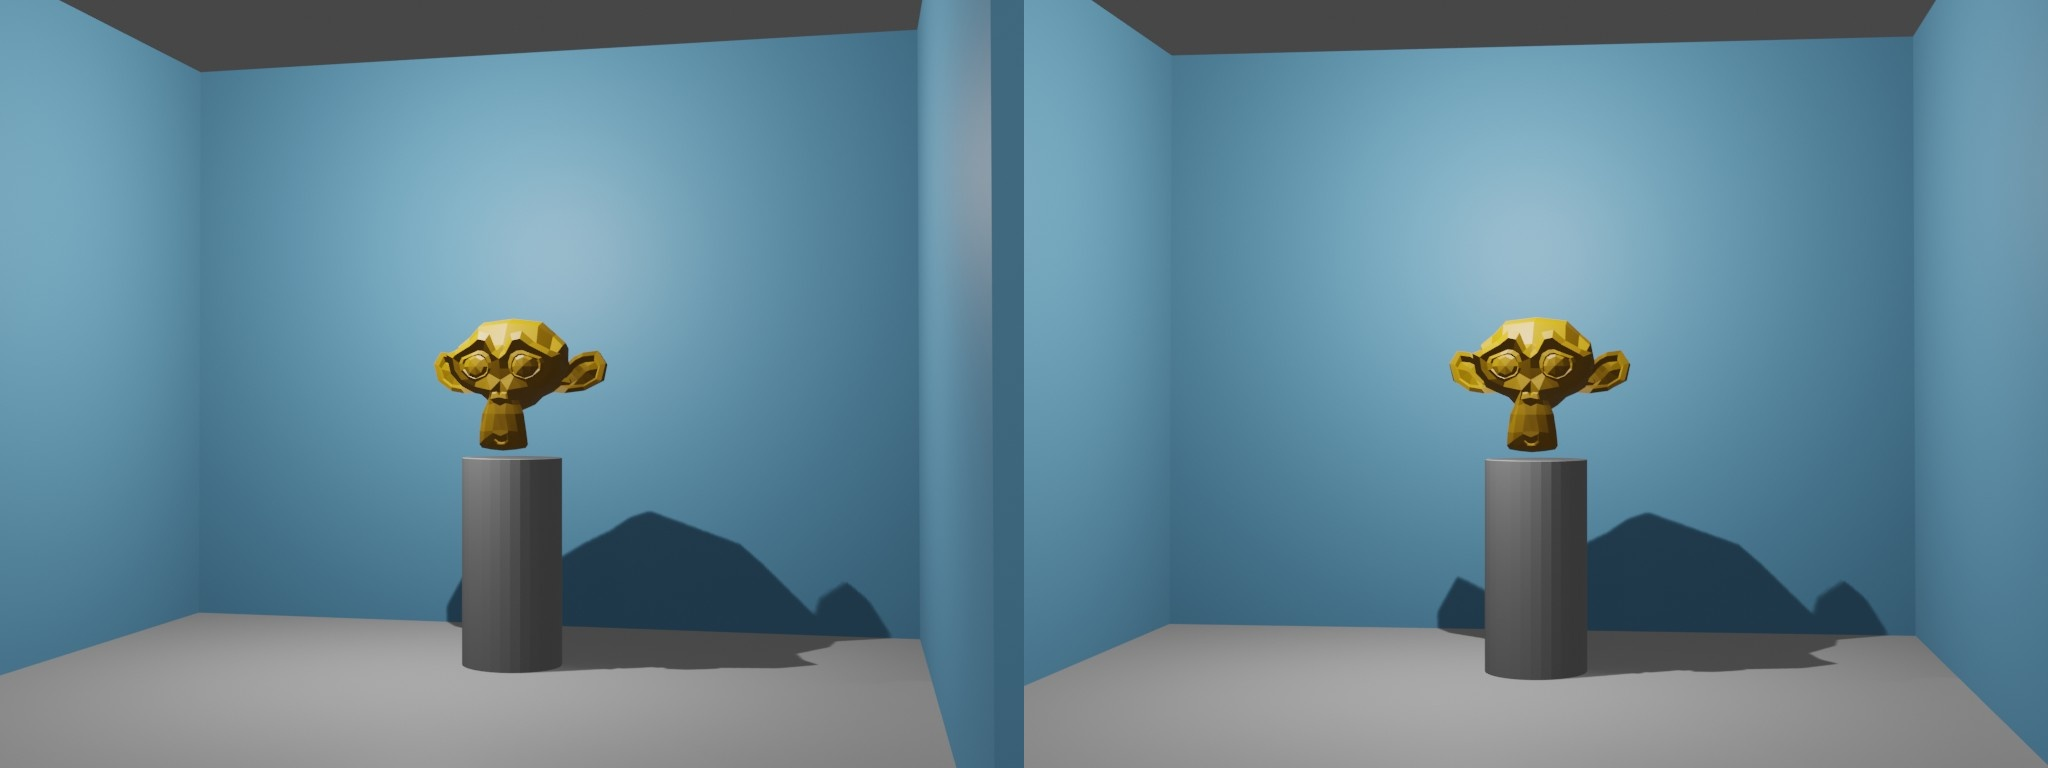
\includegraphics[width=\textwidth]{img/experiment2_environment_comparison_2.jpg}
		\caption{An example training image generated with the help of Blender.}
	\end{subfigure}
	~ 
	\begin{subfigure}[t]{\textwidth}
		\centering
		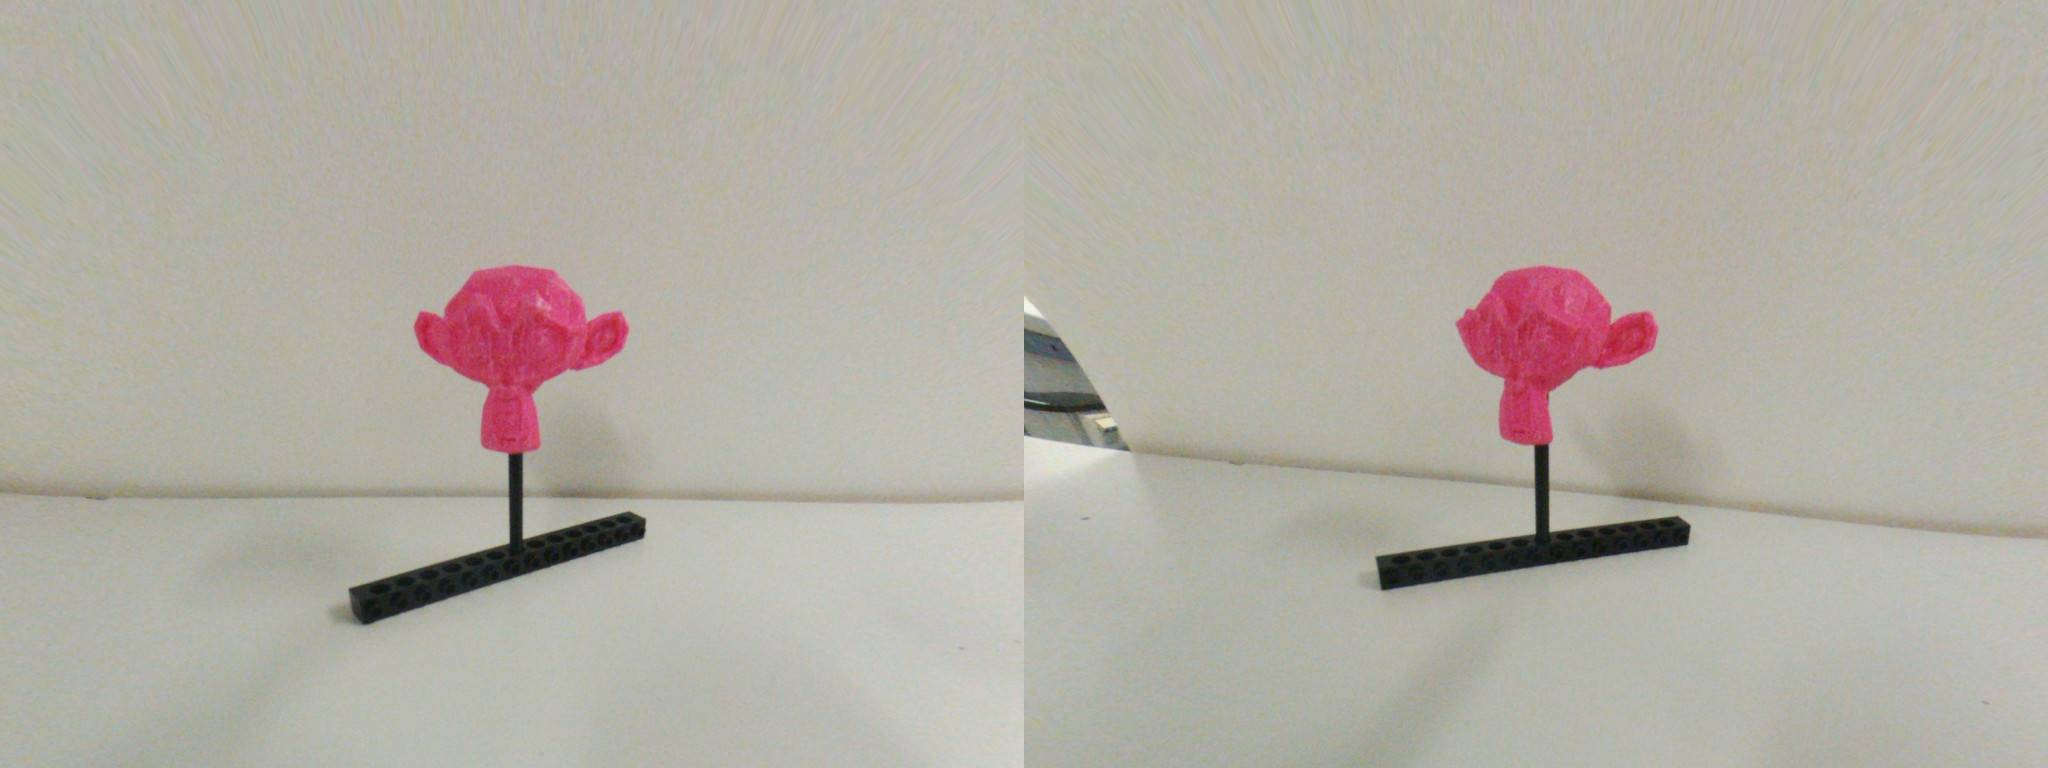
\includegraphics[width=\textwidth]{img/experiment2_environment_comparison_1.jpg}
		\caption{The two modified images of the 3D printed monkey head taken with the Parrot Bebop 2.}
	\end{subfigure}
	\caption{Image pairs of the monkey head.}
	\label{pic:experiment2_environment_comparison}
\end{figure*}

\section{Results}

\filbreak